\chapter{Business Case}
\section{Summary}
\subsection{Introduction}
The project is conducted for learning purposes, as part of a course in the IT University of Copenhagen. The goal of the project is to help DANX achieve its business goals by suggesting one or more solutions to the problem described below. The result of the project is presented in this document, which purpose is to provide a reasoned basis for a decision for whether the suggested solutions should be implemented. The reasoning is based on company documents and interviews with employees.
\subsection{Problem definition}
The employees of DANX can not access error reports from a specific customer, because some of the reports are not documented and the current system does not allow reports to be retrieved within a satisfactory time frame. This hinders potential evaluation of support given to a customer.
How can employees of DANX access documentation for customer support? \\

The problem is solved if these goals are reached.
\begin{itemize}
	\item It is possible for at least one employee to retrieve documentation for customer support.
	\item The customer support documentation provides data to evaluate how fast it is done, who it is done by, and who receives it.
	\item The solution does not increase the mean response time of customer support.
\end{itemize}

\subsection{Scope}
The scope of the project includes internal communication, not communication with customers and others outside of DANX. In other words this means that customers will still have the same high degree of service and availability from all IT-staff, because the proposed solutions do not seek to change the way customers communicate with the employees of DANX. The regional departments outside denmark will not be considered for the problem or the solution.
\subsection{Information gathering}
This is a list of the activities that the sources used in the business case is based on.

\vspace{2mm}

\begin{tabular}{ | p{\dimexpr.20\textwidth-3\tabcolsep} || p{\dimexpr.30\textwidth-2\tabcolsep} | p{\dimexpr.50\textwidth-2\tabcolsep} | }
\hline
\rowcolor{GR}
\textbf{Activity} & \textbf{Date/Time} & \textbf{Actors}\\ \hline \hline
Interview and presentation & 24.09.2013 09:00 - 12:00 & Malene Hjarnaa, Gert Philipsen, Lasse Trier \\ \hline
Interview & 23.10.2013 10:00 - 10:45 & Lasse Trier, Lahib \\ \hline
Interview & 13.11.2013 10:00 - 11:00 & Lasse Trier, Jakob \\ \hline
Interview & 20.11.2013 10:00 - 11:00 & Lasse Trier \\ \hline
Interview & 27.11.2013 10:00 - 11:00 & Lasse Trier \\ \hline
Interview & 29.11.2013 10:00 - 11:00 & Gert Philipsen \\ \hline
\end{tabular}

\section{In-line analysis resume}
This section describes the most important observations and arguments presented in the strategic alignment report. The purpose of the in-line analysis is to provide insight in the business strategy of the company, environment and an overview of work domains to make a reasoned decision for which work domain to research and optimize as well as solving the problem in a manner that fits the context.

\subsection{Business strategy}
The business strategy of DANX is aimed at ensuring customers get their spare parts fast and on time, while also delivering good support whenever needed.\cite{gert027}\cite{gert025}\cite{lasse012}

\subsection{Canvas}
See section~\ref{sec:business_canvas} for the business canvas.\\
Fast delivery, overnight delivery and guaranteed pre 7am\cite{gert001} delivery are key values of DANX. These values are greatly backed up by the key resources of DANX, Field Stock Locations and Pick-up/Drop-off locations.\cite{img001}

\subsection{Goals}
DANX has a goal of gaining 25-30 customers each year and increase their revenue to at least 500 million DKK and have a profit of 8-10\% of that within 3-5 years;
There is also a constant goal of delivering at least 99\% of pre 7 am deliveries on time.\cite{mail}

\subsubsection{Challenges and problems}
DANX face several challenges and problems, some of the more significant are explained here. \\
There are not currently being documented anything regarding customer support at any level.\cite{lasse010} The lack of documentation makes it cumbersome for the management of DANX to analyze problems related to customer support. This makes it hard to detect any weaknesses in the customer support which is crucial for the service level. \\
Neither the IT department nor the operational department have any KPIs\cite{gert011}, making it difficult to asses whether or not things are going as planned. It also makes it hard to figure out why it is going the way it is in the individual departments

\subsection{Environment}
In this section the competitors of DANX are being analyzed and compared to DANX. \\
The main competitor of DANX is a special service within TNT called TNT innight. Just as DANX, TNT innight provides delivery of items within 7 am the following day.\cite{webpage001} TNT has some advantages over DANX eg. that their company is larger\cite{tnt002} and they have their own flight route\cite{webpage001} from Bruxelles to Jönköping, Helsinki, Oslo, and Billund.
Their own flight routes are a major strength as this grants a better quality compared to DANX. If one of DANX flights are canceled the goods are likely to be delayed, whereas this is less likely to happen at TNT. \\
The most apparent advantage DANX has over TNT is that they offer faster customer integration.\cite{tnt001} \cite{lasse008} This makes DANX stronger when competing for customers with urgent needs. \\
Another competitor is HIT.\cite{malene001} HIT provides the same service as DANX, namely pre 7 am. delivery during the night. \\
One of HIT’s advantages is they have a lot of companies to back them up, such as posten.se and Postdanmark A/S.\cite{webpage002}\cite{webpage012} This increases the capital in the company which can make them a powerful competitor. \\
A disadvantage is that the company is newly started and thus does not have much experience compared to the existing ones on the market, which may lead to worse quality.

\subsection{Work domains}
The essential departments to focus on are are the IT department and the operations department.\\
The IT department develops, maintains and supports IT systems\cite{lasse015}, which are used in all of the departments of DANX and they are responsible integration with customers systems.\cite{lasse008} When DANX gets a new customer the IT department make sure that it are only taking a few days\cite{lasse008} before they have fully implemented the integration between IT systems of DANX and the customers IT system. They are also using a lot of resources on handling internal and customer support related to software inside DANX.\cite{lasse016}\\
The operations department is the main department, both in regards to internal coordination of packages as well as customer support requests.\cite{gert004} They propagate support requests when they are unable to fix the issues.\cite{lasse017}\\
The control tower is part of the operational department and serves as a reliable contact for their customers and ensures that any problems that may hinder delivery of spare parts are addressed.\cite{gert004}\\

\section{In-depth analysis resume}
This section describes the most important observations and arguments presented in the In-depth analysis report.~\ref{chap:indepthreport} The purpose of the in-depth analysis report is to provide insight into the chosen work domain, which is used as a basis for suggesting and asserting solutions.

\subsection{Key players}
This section describes the persons that have the most significant impact on the project.

\subsubsection{Lasse Trier}
Lasse Trier is the head of IT development. He has an important role in providing competitive advantages to DANX as described in the Strategic Alignment Report in Work Domains. His impact on the project is significant, because he provides solutions to customer problems.

\subsubsection{Gert Philipsen}
Gert Phillipsen is the head of the operational department. He is, among other things, concerned with optimization of the operational department\cite{gert015}, which makes his opinion on the project important.

\subsection{Current work practices}
When customers of DANX wants to report a problem to DANX, they contact the control tower in the majority of cases.\cite{gert004} Customers can contact employees on other levels than the employees of the control tower.\cite{gert007} The problems that the operational department can solve highly depend on the employee that takes care of the case.\cite{lasse002}\\
If the employee is not able to solve problem, it is propagated to the IT development department. Because some knowledge is acquired when trying to solve or identify the problem, it is in some cases propagated with a description, helping the IT development department solve it.\cite{gert006}\cite{lasse005}\\
The IT development department usually solves problems related to customer integrations, because they make the integrations internally in the IT development department. Lasse Trier is the primary provider of support.\cite{lahib004} Other employees of the IT department helps integrating to some extent.\cite{lahib002}\cite{lahib003}\\
Some problems from the same customer are recurring, because the problem was not solved in the first place.\cite{gert009}

\subsubsection{Problems}
The operational manager, can not supervise which customer support requests that are done and how long time it is pending. With this lack of knowledge it is complicated to optimize customer support. In the current situation, the knowledge of a specific problem can only be obtained by examining emails or talking to the employees that are responsible for solving the problem. The responsibility assignments are not documented, which complicates this further.\cite{gert012}\\
With no documentation of customer support, KPIs of customer response time can not be established.\cite{gert011} The bigger DANX grow, the harder it is for a single manager to maintain an overview of how well the customer support is doing. As one of the goals of DANX is to grow, this issue becomes increasingly relevant.

\subsubsection{Needs}
Both the IT development department and the operational department needs documentation of customer support in order to have data to base evaluation on. With no evaluation the operational manager can not know how well customer support is doing, and has no way to know where to optimize the department.
It is assumed that growth introduces additional employees and it is harder to asses an increasing number of employees’ performance without documentation. To guarantee that customer support requests are answered on-time, documentation that keep track of the request and the responsible employee is needed. It is assumed that an increasing amount of employees makes the need for employee evaluation increasingly important.

\subsection{Ideas for solutions and suggested priorities}
There has been proposed two solutions, they both share the common function of being able to create tickets with information regarding customer support requests and their status.\\
The second solution includes the added functionality of attaching solutions to tickets, and hence provides DANX with more detail in regards to what has been done to fix the reported tickets and which type of problem it was.\\
The differences are quite significant when comparing workflows, since the second solution requires employees to be able to properly identify types of problems to properly label solutions.\\
In regards to priority, the second type of solution fits what Gert Philipsen has expressed as being valuable for DANX.\cite{gert003}

\section{Solutions}
In this chapter the suggested solutions to the problem are assessed.

\subsection{Vision summaries}
Our envisioned changes can be divided into two categories, where the first category is a tailored system and the second being an off-the shelf software solution.
Short summaries of what functions each system must include is described in the following sections.

\subsubsection{Tailored system}
The tailored system is envisioned in two different degrees, where the first one is a basic version that has a lesser impact on current work practices than the second. \\
The second system has the addition of solutions to the problems and labelling to support queries that retrieve specific solutions. One of the stakeholders, Gert Philipsen, has expressed that he is interested in such an addition to the system.\cite{gert003}\\
Henceforth we shall refer to them as the basic tailored system and the extended tailored system.

\subsubsection{Off-the-shelf system}
The off-the shelf solution is a system named Kayako \cite{website005}. It is a highly customizable software solution, which is used widely by organisations.\cite{website006} \\
More detail on both systems will be provided in this chapter. First the common aspects of the systems will be described and later the specific details of the systems are explained.

\subsection{Requirements}
The next section will describe what requirements are needed to alleviate the issues which we have identified in the preliminary studies. These requirements are common for all the solutions and are needed to solve the problem. Some of the more detailed requirements are included in the solutions appendix ~\ref{chap:solutions}.

\subsubsection{High-level requirements}
\textbf{AR1} \\
The system must allow some users to evaluate customer support requests, such that the customer support performance of employees can be assessed. \\
\textbf{AR2} \\
The system must allow some of its users to view unfinished customer support requests. \\
\textbf{AR3} \\
The system must not change the way customers communicate with DANX.

\subsection{Basic tailored system}
\subsubsection{Changes in work practices}
The management at DANX will, with the proposed ticket system, be able to generate reports based on different criteria in order to evaluate the employees and work flow. To make such reports useful the management must act based on the results. In other words they must find time to optimize when a potential problem is discovered, or else the system has no advantages.\\
The employees providing the customer support has to undergo several organisational changes. The most significant change in practice is ticket creation when a customer reports a problem. This is only necessary for employees handling the customer communication. This is usually the employees of the control tower, but it can be others, like the head of the IT development department.~\ref{sec:workpractices} The receiver of the problem report must specify the customer and describe the problem, and instead of using email or phone to propagate the problem, he or she must specify a department to propagate it to.\\
The employees of a department must check for customer support requests because someone has to handle the request when it is propagated to a department. \\
Any employee providing customer support must edit a ticket if the information is erroneous or new information is acquired about the problem. Employees solving problems must mark a ticket solved after they have provided a solution to the problem.

\subsubsection{Employee qualification}
\label{subsub:basicqual}
The employees that are going to use the new system will require some new qualifications. First and foremost, all employees who do customer support, should be able to use the new functionalities of the system. In order to use it, employees have to write tickets which requires some specific qualifications. An employee must be able to identify the right customer which the ticket is regarding. The employee must be able to attach relevant e-mails and files to the ticket in order to keep all relevant data in the system. This follows an ability to write a proper description of the problem in order to give everyone who might read it a good understanding of what problem this ticket contains. The employees should also be able to identify the responsibilities of the 2 different IT departments in order to be able to propagate the tickets properly.\\
The management department of danx should be able to use the proposed IT system to complete task which can be used to get performance statistic for all of DANX customer support, the individual departments performance or the performance of specific employees. It should also be possible to investigate which customers require most support.\\
In order to do this they should be able to use search filters in the program to help them find the data required. These filters should include the functionality eg. to find response times for an employee, find out which tickets are being propagated from the IT department to IT support and vice versa, find tickets based on timeframe, response status for companies and the percentage of tickets which a department have handled/propagated.

\subsection{Extended tailored system}
This section contains additional information about the extended system. The requirements, changes in work practices and qualifications described above also applies to this system. The additional requirements for the extended system is included in the soultions appendix ~\ref{chap:solutions}.

\subsubsection{Changes in work practices}
Employees that provide customer support can with the addition of the extended system find solutions to problems, which changes the workflow. Instead of propagating or solving the problem directly, the employee might search for solutions to problems first, and reflect in the problem description that such a search has been done, if it is propagated. When a problem is resolved the ticket must be updated with the given solution found.

\subsubsection{Employee qualification}
\label{subsec:qualification}
In addition to the qualifications described in~\ref{subsub:basicqual} the employees that solve customer problems and therefore close tickets must acquire some additional qualifications to use the extended system.
If the problem is not correctly labeled, they must provide the correct label to make search for the solution easier. This requires that the employee knows the labels that relate to the problem that they are solving. The employee must document the solution in the form of text and possibly references to files and emails in such a way that another employee with the same problem can solve a similar problem from the description.\\
All users of the system must be able to use the functionality to search for solutions, and have a common understanding of the problems that each label covers.

\subsection{Off-the-shelf system}
The off-the-shelf solution, Kayako\cite{webpage005}, can be used as the basic or extended solution, because its functionality covers all the requirements described in the previous sections. Hence the changes in work practices are the same as the system that its functionality is similar to. For the assessment of the system in the following sections, it is assumed that the functionality used is as the extended system.
The project will not account for the SaaS\footnote{SaaS is Software as a Service, meaning it is hosted online by another company, who also maintain it.} solution with a periodic payment.

\subsubsection{Employee qualification}
The off-the-shelf solution distinguishes itself from the tailored solutions in the sense that more employee training is required. This is due to the complexity of the system.
Employees might have a hard time identifying what is relevant to their task, when its cluttered with a lot of unnecessary items.\cite{webpage007} \\
The reports generated by the system must be coded by someone from the IT development department, using a “Kayako query language”. This language will needed to be learned in order to update/add the reports. \\
A person should also be responsible for configuring the solution once it is bought. This is not a service kayako offers.\cite{webpage008} This can be a hideous task due to vast amount of configurable options in the solution.

\subsection{Advantages}
The management at DANX will, with the proposed ticket system, be able to generate reports based on different criteria in order to evaluate the employees and work flow. The reports can for example be used to evaluate the following points:
\begin{itemize}
	\item How fast the individual employees answer different types of problems. This enables for ongoing training of the employees.
	\item Which problems an employee is able to solve. Also enables for ongoing training of employees and ultimately makes employees able to solve instead of propagate problems.
	\item Detect if the employees propagate the tickets to the correct departments and correct the employees if they do not.
	\item Find unresolved tickets, in order to fix the problem within an acceptable timeframe. This should increase customer satisfaction as well as response times.
	\item Detect if multiple customers have the same problem and make a generic solution if it is needed.
\end{itemize}
The customer support KPIs can be used to make sale to potential customers more likely because some of them demand documentation for customer support.\cite{bob001}

\subsubsection{Specific for extended tailored system}
If the advanced ticket system is chosen, it is, in addition to the simple ticket system, possible to evaluate the following points:
\begin{itemize}
	\item Detect how fast a certain type of problem, determined by a tag in the ticket system, is answered.
	\item Investigate where certain types of problems are solved, thereby possibly cutting unnecessary links away from the propagation chain.
	\item Detect if an employee is unable to fix a problem that they are supposed to be able to solve.
	\item Find a solution to a problem already solved and thereby save time.
\end{itemize}
As an additional advantage, new employees might be easier to train without actual customer support practice, because they can study problems and related solutions to be better prepared for the challenges that they might face in the future.

\subsubsection{Specific for off-the-shelf}
The off-the-shelf solution also runs in a browser (and is available as a mobile app), hence there is no requirements to the computer the employee is working on, except that it has an up-to-date browser.

\subsection{Disadvantages}
Besides the advantages, the ticket system will inevitably have some disadvantages. The disadvantages include but is not limited to:

\subsubsection{Common for all system}
\begin{itemize}
	\item Employees must learn to use the system.
	\item It takes extra time to create and update the tickets.
\end{itemize}

\subsubsection{Specific for extended tailored system}
This disadvantage is in addition to the ones described above.\\
The employees who solves the problem must document the solution to the problem. This can require additional time for important employees. The time of employees that solve the most problems of a department probably provides more value per hour for DANX, and because it is the solver of the problem that has to document it, it can be time of higher value that is spent.

\subsubsection{Specific for off-the-shelf system}
The following disadvantage applies for the off-the-shelf system, in addition to the disadvantages described above. Learning to use the system might take longer time because the additional functionality of Kayako makes the UI more cluttered and less user friendly.\\
Should DANX require additional functionality at some point, the system may not support this, and DANX is dependant on the provider to implement this.\\
The system may also be a bit of an overkill if used as a basic solution. Seeing the solution is originally made for providing support, the employee will have to solve/close a ticket every time they create a new one.

\subsection{Finances}
There has been selected a company cost of capital at 7\% since the interest rate is approximately 0.125\% \cite{bank001} and that DANX is 20 years old\cite{webpage010}. This allows the company to get more profit from the invested money than just putting them in the bank. The explanations for the costs and benefits are included in the solutions appendix ~\ref{chap:solutions}.

\subsubsection{Benefits}
In our cost benefit analysis we have included the following benefits:
\begin{itemize}
\item Customer loss avoidance
\item Faster solution to problems
\item More sale
\item Less time writing emails
\end{itemize}

\subsubsection{Cost}
This is the costs that has been identified.
\begin{itemize}
\item Initial investment
\item Staff training
\item Support/updates
\item Additional time spent on documentation
\item Additional time spent on analysing
\end{itemize}

\subsubsection{Cost benefit charts}
\label{subsub:cost_benefit_charts}
\textbf{Tailored basic solution}\\
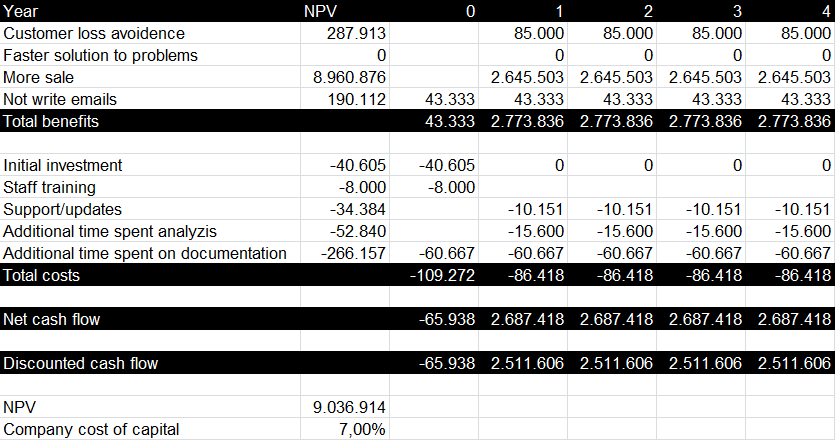
\includegraphics[width=\textwidth]{img/CostBenefit_TailoredBasic2}\\
\vspace{2mm}

\textbf{Tailored extended solution}\\
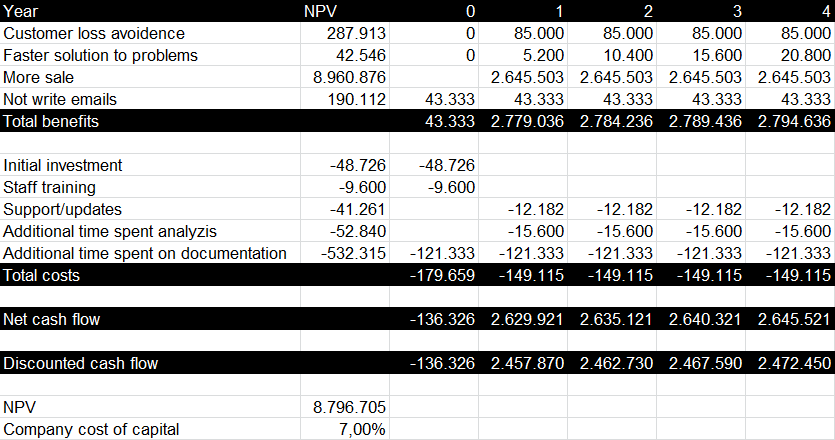
\includegraphics[width=\textwidth]{img/CostBenefit_TailoredExtended2}\\
\vspace{2mm}

\newpage
\textbf{Off-the-shelf solution}\\
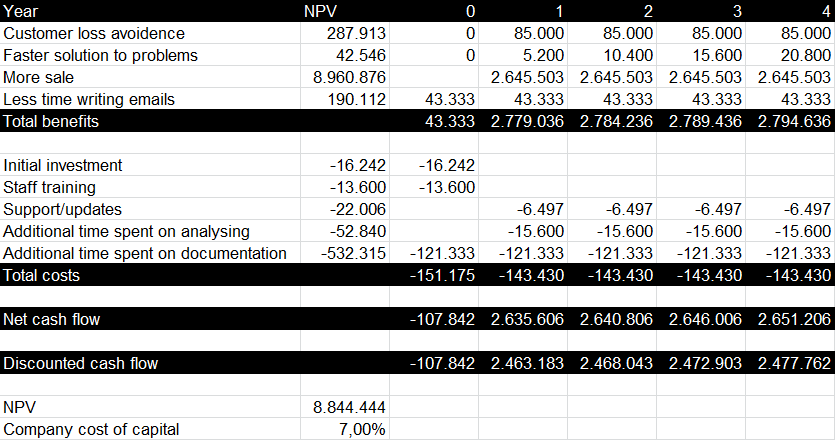
\includegraphics[width=\textwidth]{img/CostBenefit_Off-the-shelf2}

\subsubsection{Conclusion}
When evaluating the cost-benefit analysis it is important to look at the net present value. For the Kayako this value is 8,844,444. For the extended tailored solution this value is 8,796,705, and for the basic tailored solution it is 9,036,914.\cite{img002}\cite{img003}\cite{img004}
The NPV\footnote{Net Present Value} describes a value discounted back to its present value, so that its interest rate is not accounted for. The basic tailored solution suggest the tailored basic version as it has the highest NPV.\\
In this analysis it is not possible to look at the net cash flow and compare the payback period as it is the same in every year, namely year 1.\\
In this cost benefit analysis we have chosen not to include roll out, integration to other systems, and data conversion. This is because There are no other systems depending on this data, and that it is not possible to convert old data, since some of it is not available (for example phone calls). Time is not a critical factor for the project, hence why there is no roll-out cost. With that in mind the benefits takes into account that DANX does not have sufficient data to be able to use the system to its fullest before it has been live for at least a year.

\subsection{Implementation strategy}
The strategy for creating and implementing the system is included in section~\ref{sec:implementation_strategy}.
